\chapter{Implementación Multicore}

La implementación multicore aprovecha la capacidad de procesamiento de equipos con múltiples núcleos mediante el módulo \texttt{multiprocessing} de Python. A diferencia de la versión secuencial, esta implementación distribuye la evaluación de candidatos entre varios procesos independientes, reduciendo significativamente el tiempo total de ejecución.

El código fuente principal se encuentra en:

\begin{center}
\texttt{code/python/multicore.py}
\end{center}

\section{Objetivo}

El propósito de esta implementación es paralelizar la evaluación de candidatos utilizando los múltiples núcleos disponibles en la CPU, manteniendo exactamente la misma lógica de procesamiento que la versión secuencial.

Los resultados obtenidos deben coincidir con la línea base, variando únicamente el tiempo de ejecución.

\section{Estrategia de Paralelización}

La evaluación de cada candidato es completamente independiente del resto, por lo que el problema presenta un alto grado de paralelismo.

La estrategia implementada consiste en dividir el conjunto total de candidatos entre varios procesos trabajadores, los cuales realizan la evaluación de manera simultánea.

Cada proceso calcula su mejor solución local y posteriormente el proceso maestro determina el mejor resultado global.

\section{Modelo Maestro--Trabajadores}

La Figura \ref{fig:multicore_architecture} muestra el esquema de paralelización implementado.

\begin{figure}[H]
\centering
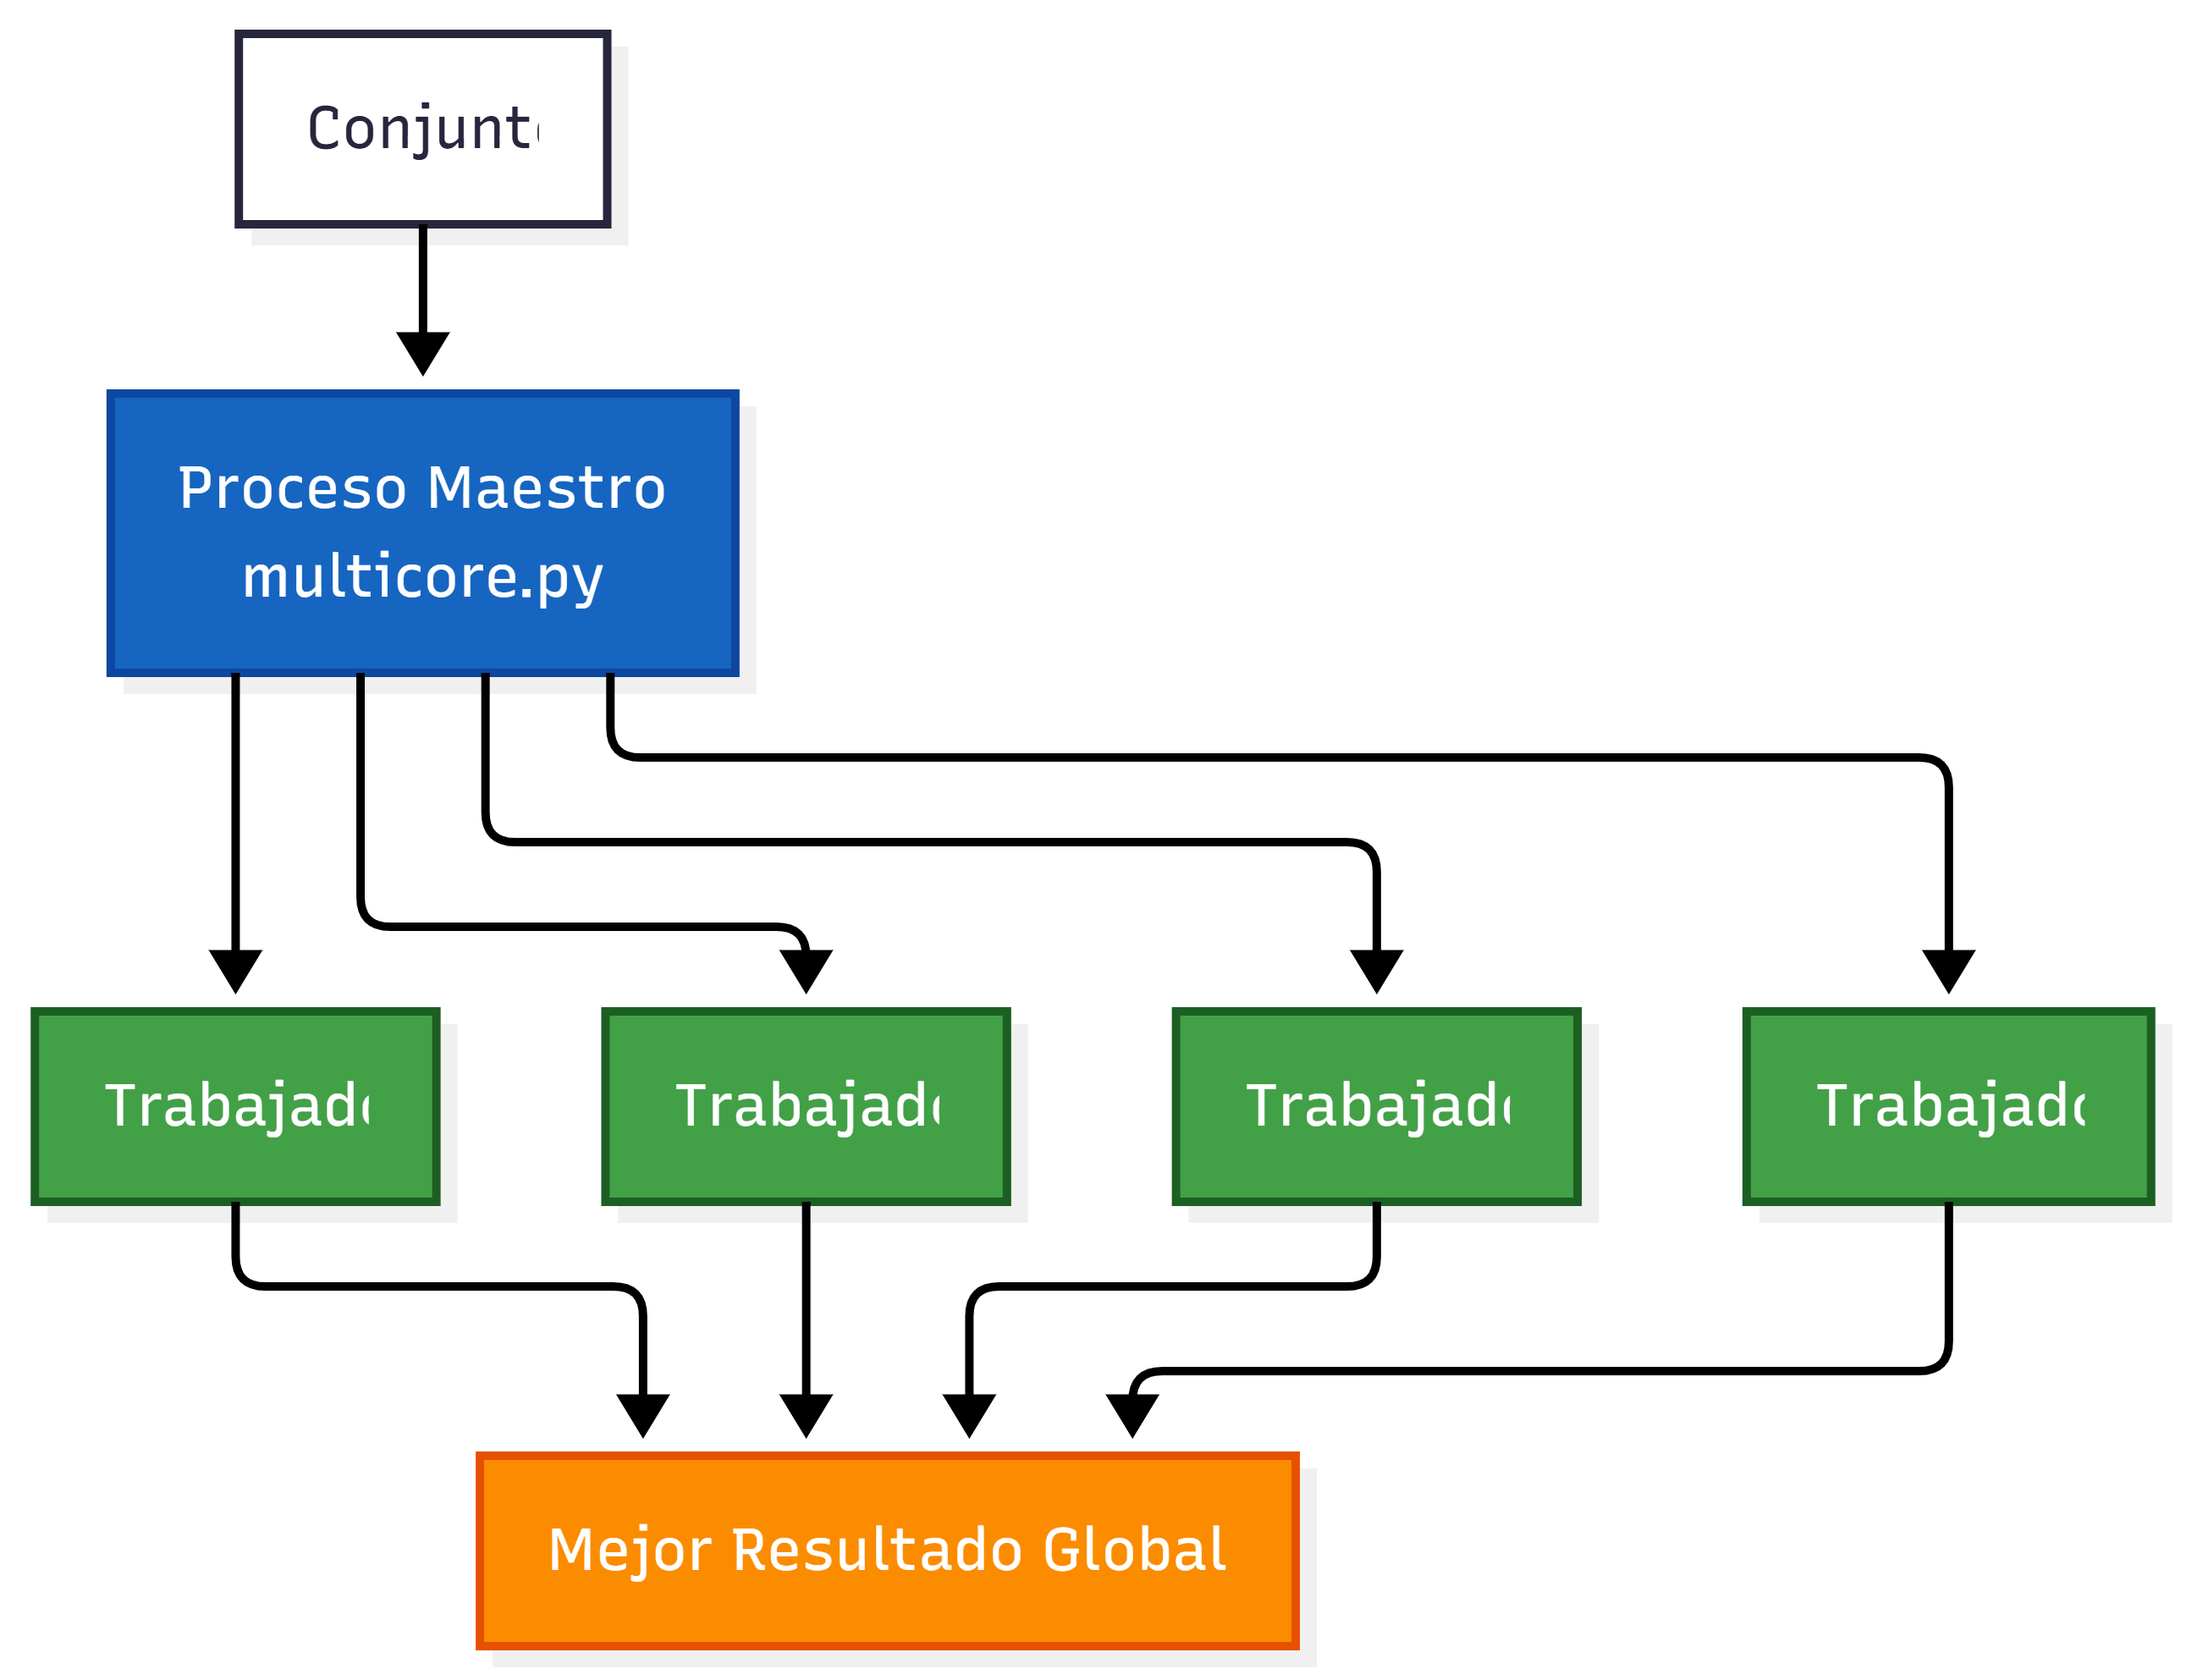
\includegraphics[width=.90\textwidth, height=0.5\textheight, keepaspectratio]
{figuras/implementaciones/03_arquitectura_multicore.png}
\caption{Arquitectura maestro--trabajadores de la implementación multicore.}
\label{fig:multicore_architecture}
\end{figure}

El funcionamiento puede resumirse de la siguiente manera:

\begin{itemize}

\item El proceso maestro genera la lista de candidatos.

\item Los candidatos se dividen en bloques de tamaño similar.

\item Cada bloque es asignado a un proceso trabajador.

\item Cada trabajador calcula su mejor valor de ROC-AUC.

\item El maestro recopila los resultados parciales.

\item Finalmente se determina el mejor candidato global.

\end{itemize}

\section{Flujo de Ejecución}

La Figura \ref{fig:flujo_multicore} resume el flujo seguido durante la ejecución paralela.

\begin{figure}[H]
\centering
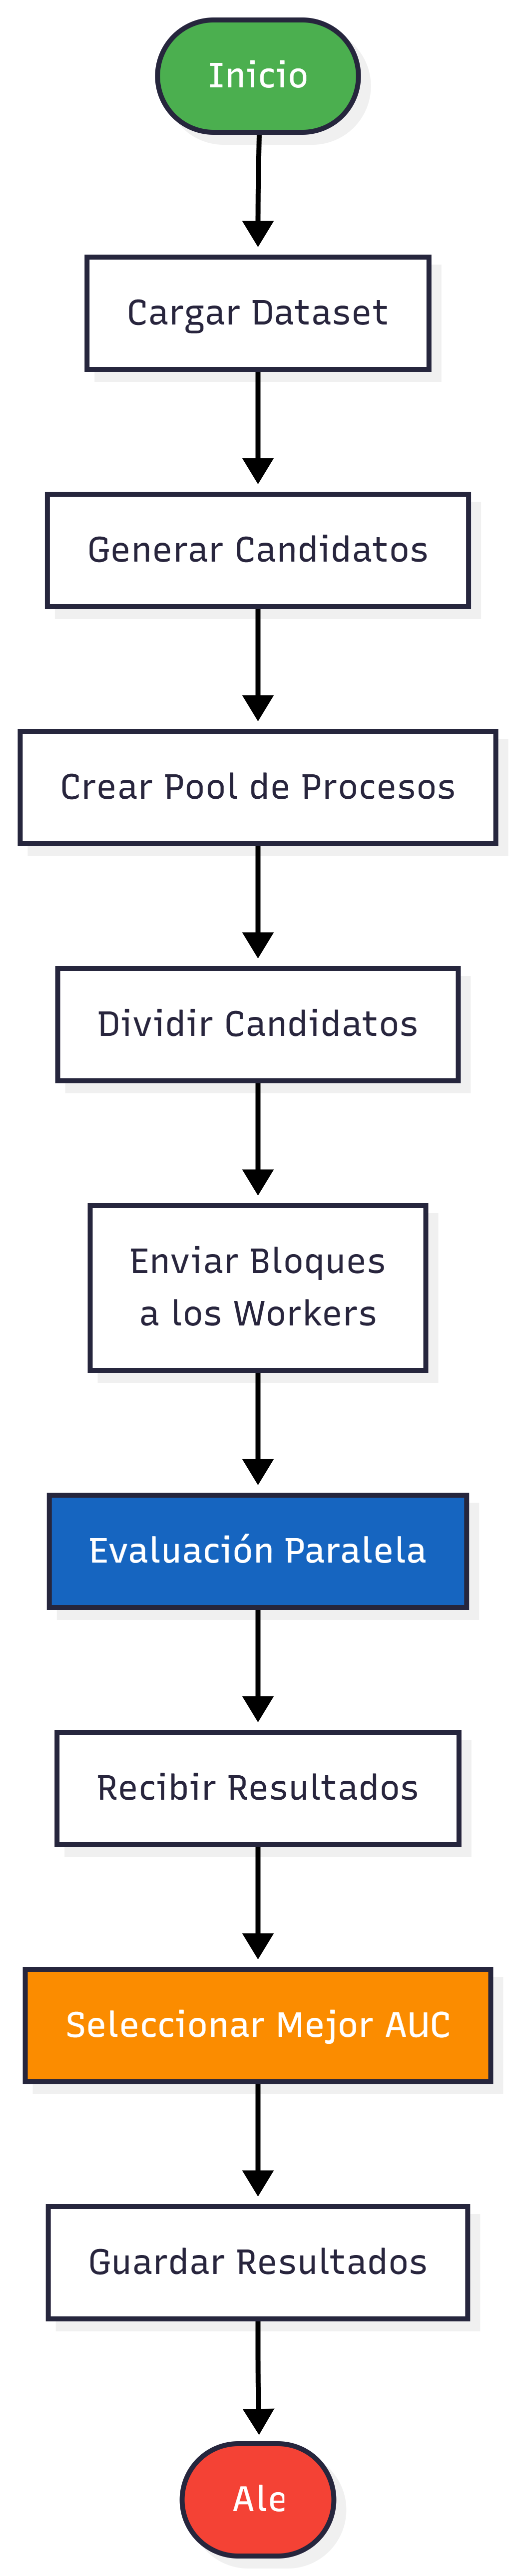
\includegraphics[width=.85\textwidth, height=0.5\textheight, keepaspectratio]
{figuras/implementaciones/04_flujo_multicore.png}
\caption{Flujo de ejecución de la implementación multicore.}
\label{fig:flujo_multicore}
\end{figure}

El procesamiento sigue las siguientes etapas:

\begin{enumerate}

\item Cargar el conjunto de datos.

\item Crear el conjunto de candidatos.

\item Inicializar el \texttt{Pool} de procesos.

\item Distribuir los bloques entre los trabajadores.

\item Evaluar los candidatos en paralelo.

\item Recopilar los mejores resultados locales.

\item Seleccionar el mejor candidato global.

\item Registrar las métricas experimentales.

\end{enumerate}

\section{Pseudocódigo}

El algoritmo implementado puede resumirse mediante el siguiente pseudocódigo.

\begin{lstlisting}
cargar_dataset()

generar_candidatos()

crear_pool()

dividir_candidatos()

parallel_map(evaluar_bloque)

combinar_resultados()

guardar_mejor_solucion()
\end{lstlisting}

\section{Complejidad Computacional}

La complejidad teórica continúa siendo

\[
O(K \times N \times M)
\]

No obstante, al distribuir los candidatos entre \(P\) procesos, el tiempo efectivo puede aproximarse por

\[
O\left(\frac{K \times N \times M}{P}\right)
\]

descontando el costo asociado a la creación de procesos y la sincronización de resultados.

\section{Ventajas}

La implementación multicore ofrece las siguientes ventajas:

\begin{itemize}

\item Aprovechamiento de múltiples núcleos del procesador.

\item Reducción significativa del tiempo de ejecución.

\item Implementación sencilla mediante \texttt{multiprocessing}.

\item Conservación de la misma lógica utilizada por la versión secuencial.

\end{itemize}

\section{Limitaciones}

Entre las principales limitaciones se encuentran:

\begin{itemize}

\item Sobrecosto asociado a la creación de procesos.

\item Consumo adicional de memoria.

\item Comunicación entre procesos mediante serialización.

\item Escalabilidad limitada por el número de núcleos físicos disponibles.

\end{itemize}

\section{Evidencia Experimental}

La Figura \ref{fig:ejecucion_multicore} presenta una ejecución de muestra de la implementación multicore durante los experimentos realizados.

\begin{figure}[H]
\centering
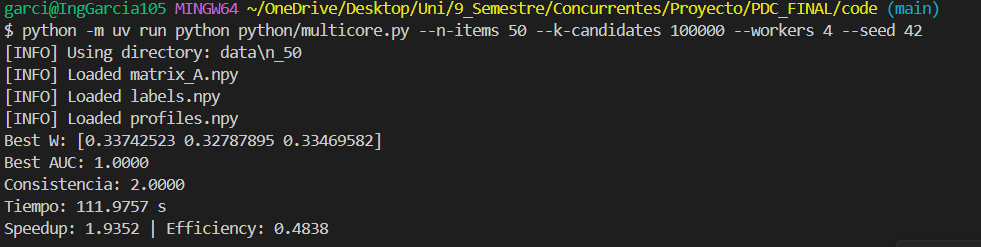
\includegraphics[width=.95\textwidth, height=0.45\textheight, keepaspectratio]
{figuras/capturas/multicore.png}
\caption{Ejecución de muestra de la implementación multicore.}
\label{fig:ejecucion_multicore}
\end{figure}

Las Figuras \ref{fig:multicore_prueba_01} a \ref{fig:multicore_prueba_05} presentan los resultados de las pruebas experimentales realizadas.

\begin{figure}[H]
\centering
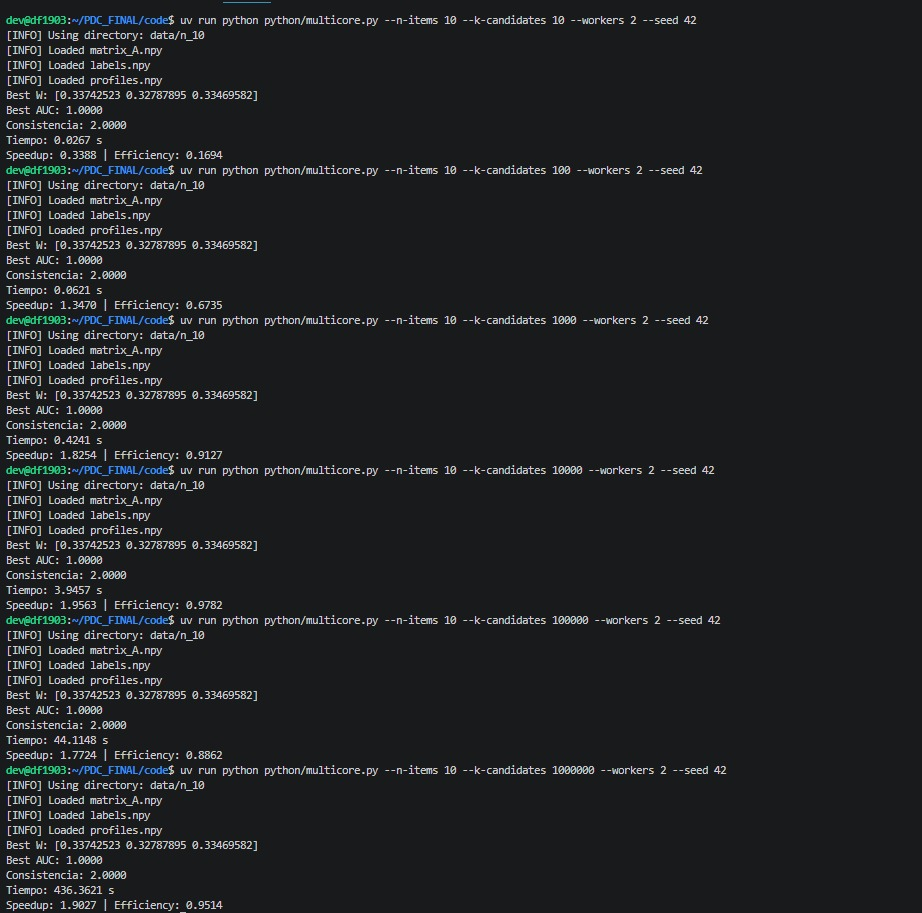
\includegraphics[width=.95\textwidth, height=0.45\textheight, keepaspectratio]
{figuras/capturas/multicore_01.png}
\caption{Prueba experimental 1 -- Implementación multicore.}
\label{fig:multicore_prueba_01}
\end{figure}

\begin{figure}[H]
\centering
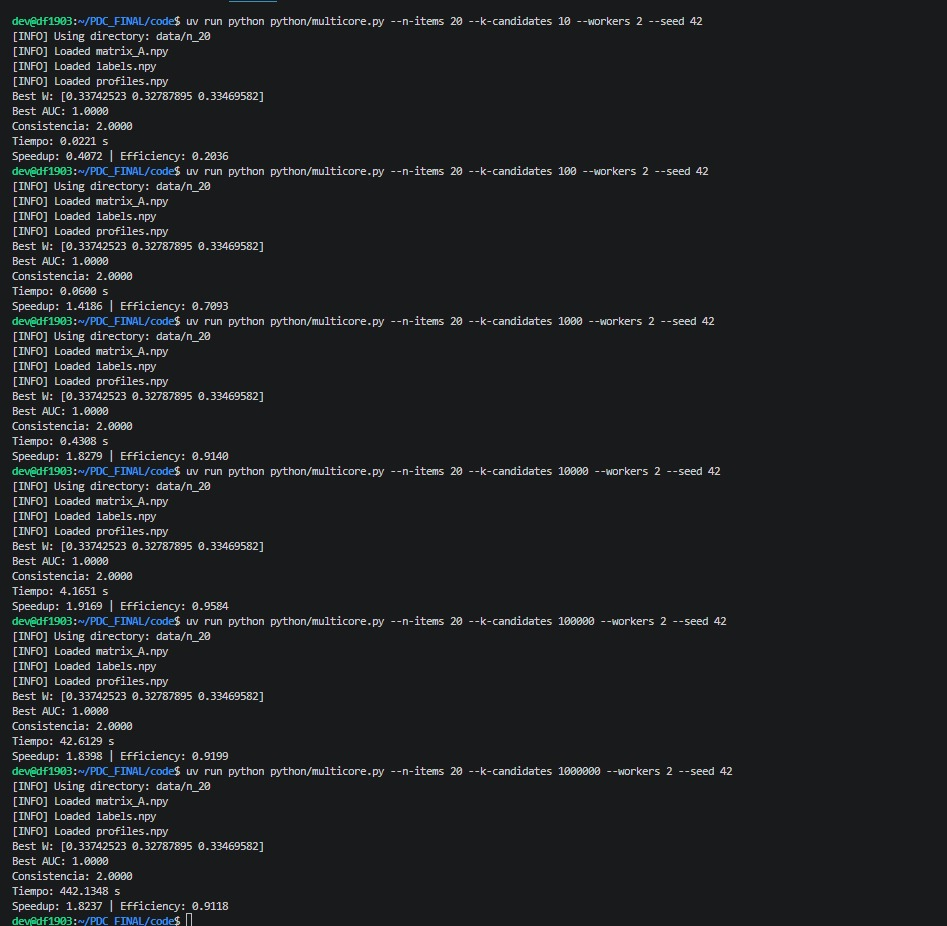
\includegraphics[width=.95\textwidth, height=0.45\textheight, keepaspectratio]
{figuras/capturas/multicore_02.png}
\caption{Prueba experimental 2 -- Implementación multicore.}
\label{fig:multicore_prueba_02}
\end{figure}

\begin{figure}[H]
\centering
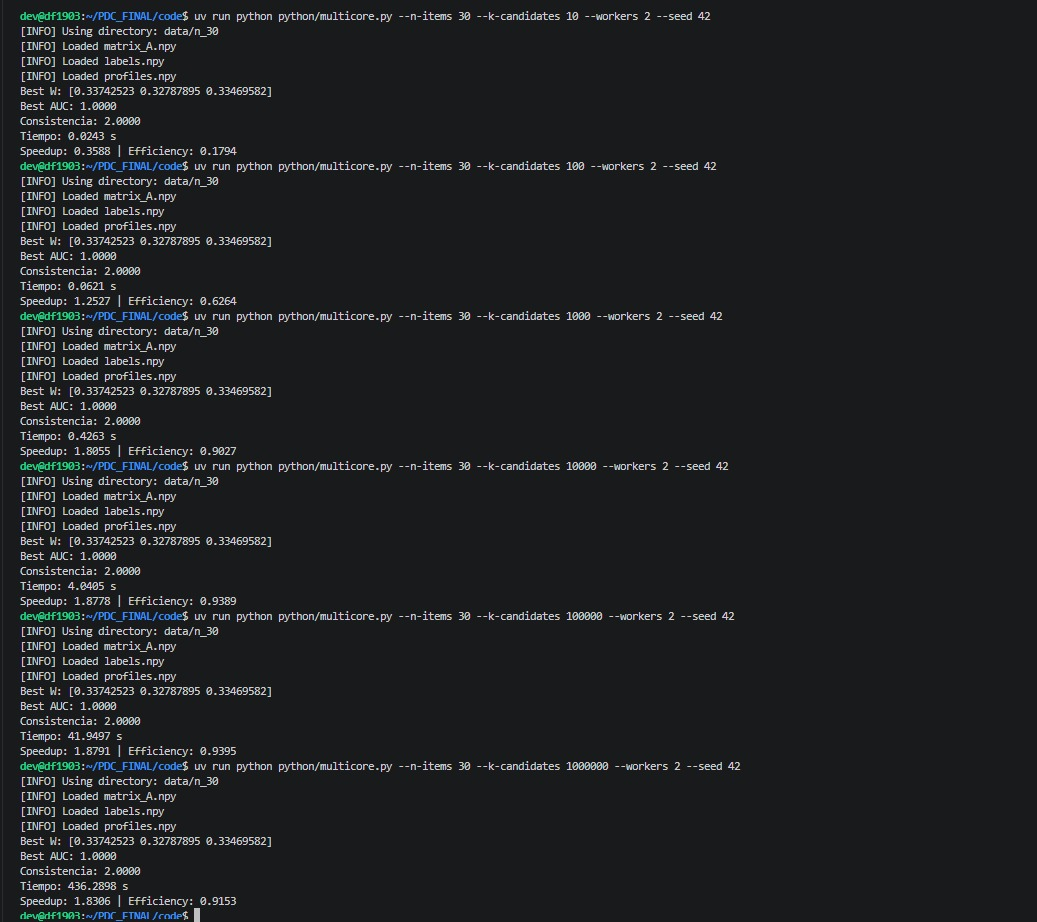
\includegraphics[width=.95\textwidth, height=0.45\textheight, keepaspectratio]
{figuras/capturas/multicore_03.png}
\caption{Prueba experimental 3 -- Implementación multicore.}
\label{fig:multicore_prueba_03}
\end{figure}

\begin{figure}[H]
\centering
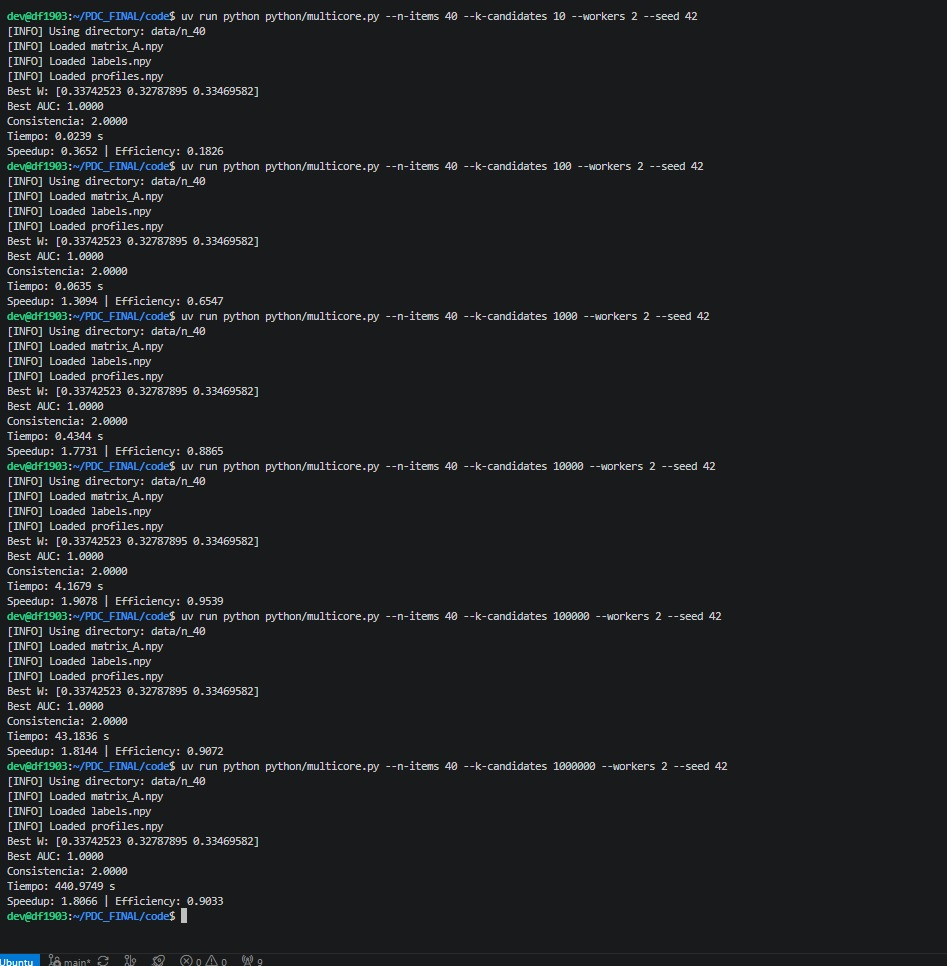
\includegraphics[width=.95\textwidth, height=0.45\textheight, keepaspectratio]
{figuras/capturas/multicore_04.png}
\caption{Prueba experimental 4 -- Implementación multicore.}
\label{fig:multicore_prueba_04}
\end{figure}

\begin{figure}[H]
\centering
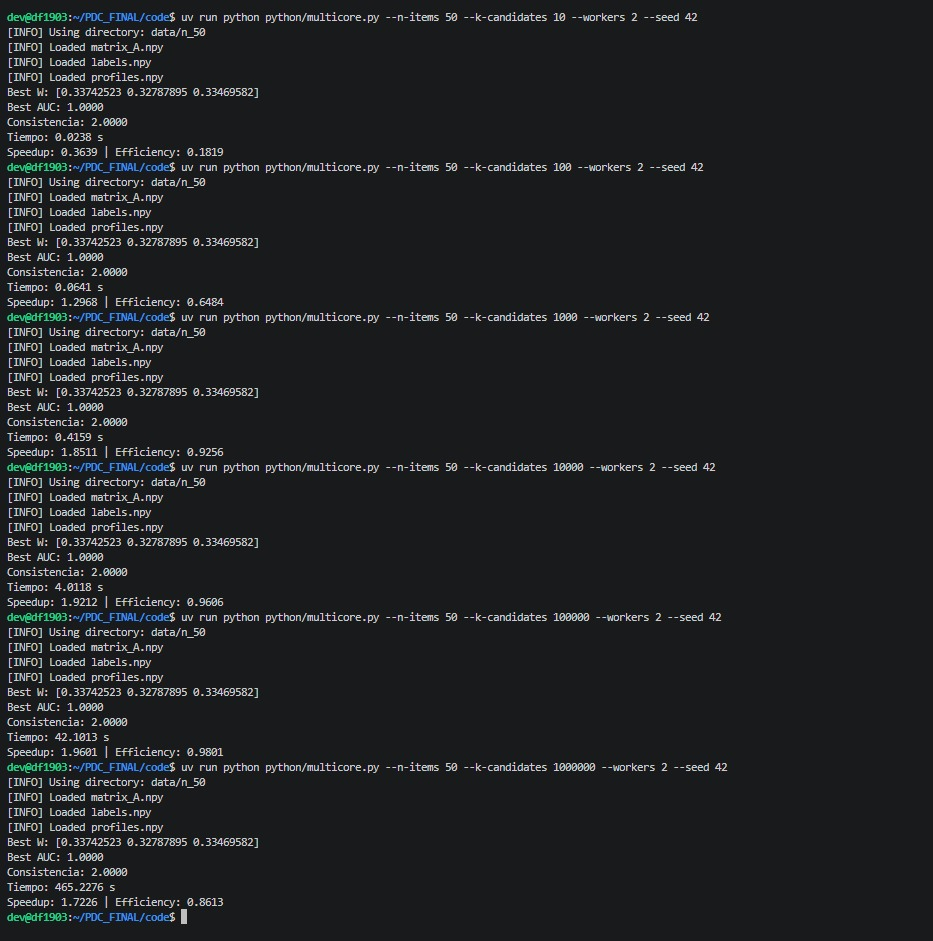
\includegraphics[width=.95\textwidth, height=0.45\textheight, keepaspectratio]
{figuras/capturas/multicore_05.png}
\caption{Prueba experimental 5 -- Implementación multicore.}
\label{fig:multicore_prueba_05}
\end{figure}

Durante la ejecución se registra automáticamente el tiempo total de procesamiento, el mejor valor de ROC-AUC encontrado y la información correspondiente a los procesos utilizados.

\section{Comparación con la Implementación Secuencial}

La implementación multicore conserva exactamente la misma lógica del algoritmo secuencial, garantizando que el mejor valor de ROC-AUC obtenido sea idéntico en ambas versiones.

La diferencia principal radica en la distribución de la carga de trabajo entre varios procesos, permitiendo reducir considerablemente el tiempo de ejecución para conjuntos de datos de gran tamaño.